% =============================================================================
% Manuscript v2 (reframed around execution rules). Springer Nature research-article
% structure. Previous version (FRESCO-centred): paper/archive/fresco_manuscript_v1.tex
%
% Template note: standard article class so it compiles anywhere (tectonic/pdflatex).
% For submission switch to the official Springer Nature template (sn-jnl.cls v3.1):
%   \documentclass[pdflatex,sn-mathphys-num]{sn-jnl}
% and map \title/\author/\abstract/\keywords/Declarations to the template macros.
%
% STATUS: working manuscript. All empirical results are SYNTHETIC (simulator and
% slot-level Monte Carlo with known ground truth). Real-agent results are [TO RUN].
% =============================================================================
\documentclass[11pt]{article}
\usepackage[a4paper,margin=2.4cm]{geometry}
\usepackage[T1]{fontenc}
\usepackage{lmodern}
\usepackage{amsmath,amssymb,amsthm}
\usepackage{booktabs,tabularx,array}
\usepackage{graphicx}
\usepackage[numbers,sort&compress]{natbib}
\usepackage{algorithm}
\usepackage{algpseudocode}
\usepackage{xcolor}
\usepackage{tikz}
\usetikzlibrary{arrows.meta,positioning,fit,backgrounds}
\usepackage[font=small,labelfont=bf]{caption}
\usepackage[section]{placeins}
\usepackage[colorlinks=true,linkcolor=blue!50!black,citecolor=blue!50!black,urlcolor=blue!50!black]{hyperref}
\graphicspath{{../figures/}}

\newtheorem{theorem}{Theorem}
\newtheorem{proposition}[theorem]{Proposition}
\newtheorem{assumption}{Assumption}
\theoremstyle{definition}
\newtheorem{definition}{Definition}
\newcommand{\todo}[1]{\textcolor{red!70!black}{[#1]}}
\newcommand{\E}{\mathbb{E}}
\newcommand{\bhat}{\hat b}
\renewcommand{\algorithmicrequire}{\textbf{Input:}}

\title{Execution Semantics Are Statistics:\\ Rules for Valid Security Evaluation of LLM Agents on Unreliable Infrastructure}
\author{\todo{AUTHORS AND AFFILIATIONS TO BE INSERTED}}
\date{Working manuscript v2, 18 October 2026 --- simulation results only; real-agent results pending}

\begin{document}
\maketitle

\begin{abstract}
\noindent\textbf{Purpose.} Security evaluations of LLM agents confirm vulnerabilities statistically, by repeating stochastic agent episodes, and run them on distributed harnesses whose defaults---at-least-once delivery, retry with fresh randomness, results consumed as they arrive, worker-local configuration---were designed for throughput. We ask whether these execution semantics preserve the error guarantees of the reported results.
\textbf{Methods.} We state six execution rules and prove that, under them, both sequential (e-process) and fixed-sample (exact binomial) confirmation keep their nominal false-confirmation level under message loss, duplication, reordering, crashes, partitions and elastic membership. We show by construction that each corresponding default can break validity, and evaluate the rules in a deterministic fault-injection simulator and slot-level Monte Carlo with known ground truth.
\textbf{Results.} At nominal level 0.05, executor defaults raised the false-confirmation probability of sequential confirmation to 0.08--0.13 and of fixed-sample confirmation to 0.11--0.999; with the rules it stayed at or below 0.035 in every configuration. A reference implementation scaled 25$\times$ on 32 workers at about 3.5 messages per episode. Auditing the counterfactual-margin estimator of MARGIN-Bench, we found it exceeds its nominal error (0.257) and give an exact repair. A shared coordinator gave no speed-up over independent runs with a split budget, and anytime-valid confirmation cost 2--5 points of power against the repaired fixed design.
\textbf{Conclusion.} Execution semantics belong in the statistical protocol of agent security evaluation. Real-agent measurements are specified but not yet executed.
\end{abstract}

\noindent\textbf{Keywords:} LLM agents; security evaluation; statistical validity; distributed systems; fault tolerance; sequential testing; e-values; reproducibility

% -----------------------------------------------------------------------------
\section{Introduction}\label{sec:intro}

Tool-using language-model agents fail securely or insecurely through \emph{actions}---an unauthorized ledger update, a forwarded secret, a privilege change---and benchmarks increasingly measure these actions in executable sandboxes~\cite{greshake2023,debenedetti2024agentdojo,zhan2024injecagent,jiang2026agentlab}. Because agents are stochastic, a single violating episode is weak evidence; best-of-$N$ attacks show that success grows with repetition~\cite{hughes2025bon}. Rigorous evaluations therefore \emph{confirm} vulnerabilities statistically: a candidate intervention is declared to violate policy with probability at least $\alpha$ only when repeated episodes support it at a stated error level~\cite{miller2024errorbars,kaur2026ceiling}. MARGIN-Bench~\cite{marginbench2026} builds a full estimand on this idea, the counterfactual safety margin
\begin{equation}
R_{s,\alpha}(M,E)=\inf\{\,c_s(\delta)\;:\;p_M(E,\delta)\ge\alpha\,\},\label{eq:margin}
\end{equation}
the cheapest intervention on attack surface $s$ whose violation probability reaches $\alpha$.

Such evaluations need $10^7$--$10^8$ agent episodes and run on distributed harnesses. The defaults of those harnesses are reasonable for throughput and harmful for statistics. A queue that redelivers a result makes one episode count twice. A retry policy that re-runs crashed episodes with fresh randomness keeps the outcomes of episodes that happened not to crash---and long, benign trajectories crash more often. Consuming results as they arrive orders evidence by latency, which depends on the outcome. Letting each worker apply its own error budget multiplies the family-wise error by the number of workers. None of these is a bug in the statistical test; each changes the data the test sees.

This paper argues that \emph{execution semantics are part of the statistical protocol} and makes the argument precise.

\paragraph{Contributions.}
\begin{enumerate}
\item[C1] \textbf{Six execution rules} (Table~\ref{tab:rules}) and proofs that, under them, sequential e-process confirmation (Theorem~\ref{thm:seq}) and fixed-sample exact confirmation (Proposition~\ref{prop:fixed}) keep their nominal error under message loss, duplication, reordering, crashes, partitions and elastic membership, for any scheduler.
\item[C2] \textbf{Necessity.} For each rule, the corresponding executor default admits executions whose false-confirmation probability exceeds the nominal level, in several cases tending to one (Theorem~\ref{thm:necessity}); we reproduce this for both test families in simulation.
\item[C3] \textbf{Audit and repair} of the MARGIN-Bench margin estimator, which as specified exceeds its nominal error five-fold; an exact repair restores validity at no efficiency cost.
\item[C4] \textbf{Cost of the rules.} A reference implementation (a single-ledger protocol) and a fault-injection evaluation showing near-linear scaling, small coordination cost and fast recovery.
\item[C5] \textbf{Estimator guidance} from preregistered comparisons: a repaired fixed design is the most powerful at a fixed budget; anytime-valid confirmation buys flexible stopping at a 2--5 point power cost; a shared coordinator is unnecessary for speed.
\end{enumerate}

\paragraph{Non-claims.} We do not propose a new statistical test; the inferential results we rely on are standard. We claim no certified lower bound on the margin, no Byzantine tolerance, validity only when episodes share no hidden state, and no finding about real agents: all results are synthetic, and the real-agent protocol (Section~\ref{sec:real}) is specified but not executed.

% -----------------------------------------------------------------------------
\section{Setting}\label{sec:setting}

\paragraph{Confirmation.} A generator proposes candidates $\delta_1,\delta_2,\dots$ with costs $c(\delta_j)\in\{1,\dots,K\}$. Executing candidate $j$ in \emph{slot} $k$ with randomness key $u_{j,k}$ yields the committed-violation label $Y_{j,k}=Y(\delta_j,u_{j,k})\in\{0,1\}$ of a permission-grounded oracle; $p(\delta_j)=\Pr_u[Y=1]$. A \emph{confirmation procedure} declares candidate $j$ confirmed when its evidence rejects $H_j:p(\delta_j)\le\alpha$ at level $a_j$; the reported margin is $\bhat=\min\{c(\delta_j):j\text{ confirmed}\}$ and the target is
\begin{equation}
\Pr(R_{s,\alpha}>\bhat)\le\varepsilon,\label{eq:G1}
\end{equation}
implied by the no-false-witness property $\Pr(\exists j\text{ confirmed}:p(\delta_j)\le\alpha)\le\varepsilon$. We consider two families: \emph{fixed-sample} confirmation (an exact binomial test on a predetermined number $n$ of slots) and \emph{sequential} confirmation (a betting e-process that may stop at any slot).

\paragraph{The harness.} Workers request slots, executors run one sandboxed episode per slot from an immutable snapshot, and results travel over a network that may delay, reorder, duplicate or drop messages and partition. Workers and executors fail by crashing; membership changes over time. Workers are honest (they belong to the evaluator); Byzantine behaviour is out of scope. The generator is treated as untrusted with respect to the statistics: it sees committed outcomes but never a slot's key before the slot is registered.

\begin{assumption}[Independent episodes]\label{as:a1} Keys are i.i.d.\ and independent of the generator's randomness, and episodes share no hidden state, so $Y_{j,k}$ given the registration of $j$ is Bernoulli$(p(\delta_j))$ independently across slots.\end{assumption}
\begin{assumption}[Crash independence]\label{as:a2} Whether a slot crashes may depend on its own trajectory and on infrastructure noise independent of other slots' keys. (Not needed when crashed slots are replayed with the same key.)\end{assumption}
\begin{assumption}[Oracle correctness]\label{as:a3} $Y$ is the true committed-violation label; with false-positive rate $\omega$ all guarantees concern $p+\omega(1-p)$.\end{assumption}

% -----------------------------------------------------------------------------
\section{Related work}\label{sec:related}

\paragraph{Valid inference under adaptivity.} Test supermartingales, Ville's inequality and e-values give inference valid under optional stopping~\cite{ramdas2023savi,vovk2021,grunwald2024safe}; betting confidence sequences~\cite{waudbysmith2024,howard2021}, always-valid A/B testing~\cite{johari2022}, e-value and online multiple testing~\cite{wang2022ebh,xu2024online,foster2008}, weighted error spending~\cite{genovese2006} and group-sequential designs with delayed responses~\cite{hampson2013} are mature. All assume the observation sequence is well defined. We study how a fault-prone executor \emph{produces} that sequence.

\paragraph{Statistical assurance in testing and search.} Residual-risk estimation in fuzzing~\cite{bohme2018stads,bohme2021residual}, statistical model checking~\cite{younes2006,legay2010}, scenario optimisation~\cite{campi2008}, threshold and infinitely-armed bandits~\cite{kano2019,locatelli2016,aziz2018,chaudhuri2017} and their parallel variants~\cite{hillel2013,li2020asha} bound errors of search or identification; parallel fuzzing schedulers remove redundant work for deterministic oracles~\cite{dynamiq2025}. For stochastic confirmation, redundancy and ordering become correctness issues.

\paragraph{Distributed systems.} We reuse leases~\cite{gray1989leases}, escrow~\cite{oneil1986escrow}, monotone state and coordination-freedom~\cite{shapiro2011crdt,hellerstein2020calm}, causal ordering~\cite{lamport1978,chandy1985}, list-scheduling bounds~\cite{graham1969} and task frameworks~\cite{moritz2018ray}. Treating a non-replenishable statistical budget as a cluster resource has a precedent in differential-privacy budget scheduling~\cite{luo2021privatekube}.

\paragraph{LLM agent security.} Benchmarks cover injection, tool use, long-horizon and multi-agent attacks~\cite{debenedetti2024agentdojo,zhan2024injecagent,jiang2026agentlab,tamas2025,darkside2025,mazeika2024harmbench}; counterfactual and causal analyses separate permission from apparent risk~\cite{yang2026agentboundary,mothukuri2026causaltrace}; defences enforce capabilities, provenance and delegation~\cite{debenedetti2025camel,south2025delegation,pang2019zanzibar,birgisson2014macaroons}; time-of-check-to-time-of-use flaws affect agents themselves~\cite{lilienthal2025toctou}. We are not aware of work treating the evaluation harness's execution semantics as part of the statistical protocol.

\paragraph{What is new.} Each mechanism in our rules (idempotent delivery, in-order commit, deterministic replay, leases) is established, and so is each inferential result. The contribution is the mapping between them: which executor semantics preserve or break which test assumptions, proofs for both test families, constructions showing necessity, a quantified audit of a concrete estimator, and measurements of what the rules cost.

% -----------------------------------------------------------------------------
\section{Execution rules}\label{sec:rules}

\begin{table}[!htbp]\centering\small
\caption{Execution rules, the default each one forbids, and the test families that need it.}\label{tab:rules}
\renewcommand{\arraystretch}{1.25}
\begin{tabularx}{\linewidth}{>{\raggedright}X>{\raggedright}p{4.6cm}>{\raggedright\arraybackslash}p{1.7cm}}
\toprule
Rule & Forbidden default & Needed by \\\midrule
\textbf{R1 Fresh index-keyed slots.} Key $u_{j,k}=\mathrm{PRF}_\kappa(\text{run},j,k)$, revealed only when the slot is leased. & seed sets shared across candidates and reused for selection; seeds visible to the generator & both \\
\textbf{R2 Predictable decisions.} Bets use only registration data and the committed prefix; fixed-sample tests run only on the complete slot set. & betting on or peeking at results not yet committed & both \\
\textbf{R3 Exactly-once, index-determined evidence.} Each slot has one terminal value (first write wins, fenced by a lease token); evidence is the in-order committed prefix (sequential) or the predetermined index set (fixed-sample). & at-least-once consumption; consuming results in arrival order; ``first $n$ results to arrive'' & both \\
\textbf{R4 Direction-aware imputation, no fresh retry.} A crashed slot counts as non-violating for confirmation (violating for audits); re-running is allowed only with the same key. & retry on failure with fresh randomness & both \\
\textbf{R5 One global error budget.} Every level $a_j$ is spent from a single budget, e.g.\ leases from one ledger or a fixed split $\varepsilon/W$. & each worker spending $\varepsilon$ on its own & both \\
\textbf{R6 Verifiable confirmation.} Decisions are recomputed from stored slot records, not taken from workers. & trusting worker-side decisions & both (integrity) \\
\bottomrule\end{tabularx}
\end{table}

\begin{theorem}[Sequential confirmation under the rules]\label{thm:seq}
Let candidate $j$ use the e-process $E_{j,n}=\prod_{i\le n}(1+\lambda_{j,i}(\tilde Y_{j,i}-\alpha))$ with $\lambda_{j,i}\in[0,1/\alpha)$ a function of registration data and $\tilde Y_{j,1..i-1}$, and be confirmed when $\sup_nE_{j,n}\ge1/a_j$, where $a_j$ is fixed at registration and $\sum_ja_j\le\varepsilon$ almost surely. Under Assumptions~\ref{as:a1}--\ref{as:a2} and rules R1--R5, for every generator, scheduler, stopping rule and execution order, $\Pr(\exists j:H_j\text{ true}, j\text{ confirmed})\le\varepsilon$.
\end{theorem}
\begin{proof}
Extend each candidate's slot sequence to infinity and let $E^*_{j,n}$ be the e-process on the full recorded sequence, $\mathcal G_{j,n}=\sigma(\text{registration of }j,\tilde Y_{j,1..n},\text{crash noise of slots }1..n)$. By R1 and Assumptions~\ref{as:a1}--\ref{as:a2}, $u_{j,n+1}$ is independent of $\mathcal G_{j,n}$; by R4, $\tilde Y\le Y$ pointwise; so $\E[\tilde Y_{j,n+1}\mid\mathcal G_{j,n}]\le p(\delta_j)\le\alpha$ under $H_j$, and with R2 $E^*_j$ is a non-negative supermartingale from 1. Ville's inequality conditional on registration gives $\Pr(\sup_nE^*_{j,n}\ge1/a_j)\le a_j$. By R3 the committed stream is a prefix of the full sequence, so any confirmation implies $\sup_nE^*_{j,n}\ge1/a_j$ whatever the schedule, stopping or abandonment. Summing over registrations and using R5 gives the bound $\varepsilon$.
\end{proof}

\begin{proposition}[Fixed-sample confirmation under the rules]\label{prop:fixed}
Let candidate $j$ be confirmed when $S_j=\sum_{k=1}^{n}\tilde Y_{j,k}\ge s^*_j$, where the index set $\{1,\dots,n\}$ and the level $a_j$ are fixed at registration, $\Pr(\mathrm{Bin}(n,\alpha)\ge s^*_j)\le a_j$ (equivalently, the exact Clopper--Pearson lower bound exceeds $\alpha$), the test is evaluated only when all $n$ slots are terminal, and $\sum_ja_j\le\varepsilon$. Under Assumptions~\ref{as:a1}--\ref{as:a2} and rules R1--R5 the same guarantee holds.
\end{proposition}
\begin{proof}
Given registration, $(Y_{j,k})_{k\le n}$ are i.i.d.\ Bernoulli$(p(\delta_j))$ by R1 and Assumption~\ref{as:a1}; R3 makes $S_j$ the sum over exactly these indices, each counted once; R4 gives $\tilde Y\le Y$; so $S_j$ is stochastically dominated by $\mathrm{Bin}(n,p(\delta_j))$, which under $H_j$ is dominated by $\mathrm{Bin}(n,\alpha)$. Hence $\Pr(S_j\ge s^*_j)\le a_j$, and the union bound with R5 gives $\varepsilon$. R2 forbids evaluating the test on partial sets, which would turn it into an uncorrected sequential test.
\end{proof}

\begin{theorem}[Necessity of the rules]\label{thm:necessity}
For each rule there is a fault pattern, with all other rules kept, under which the false-confirmation probability exceeds the nominal level:
\begin{enumerate}
\item \emph{R3, duplicates.} Sequential: every result applied twice yields $(E^*)^2$, and at $p=\alpha$ the error lies in $[\sqrt\varepsilon/(1+\lambda(1-\alpha)),\sqrt\varepsilon]$. Fixed-sample: duplicates displace fresh slots, shrinking the effective sample and inflating the variance of $S_j/n$.
\item \emph{R4, fresh retry.} If benign episodes crash with probability $c_0>c_1$ (the violating rate), the recorded stream is Bernoulli$\bigl(p(1-c_1)/(p(1-c_1)+(1-p)(1-c_0))\bigr)>\alpha$ at $p=\alpha$; a consistent sequential test then errs with probability tending to one, and a fixed-sample test errs with probability increasing in $n$.
\item \emph{R3, arrival order.} If violating episodes return first, the first $n$ arrivals out of $m>n$ launched, or the arrival-ordered prefix, over-represent violations; as $m\to\infty$ the error tends to one for both families.
\item \emph{R5.} $W$ workers each spending $\varepsilon$ give family-wise error $1-(1-\varepsilon_0)^W\to1$.
\item \emph{R1/R2.} Selecting candidates on a shared fixed seed set and confirming on the same seeds, or betting with knowledge of the current outcome, yields error tending to one.
\end{enumerate}
\end{theorem}
\begin{proof}
Each item is a direct construction; items 1 (sequential) and 2 follow from the stated distributions and optional stopping, item 3 from the order statistics of latencies, item 4 from independence across workers. Section~\ref{sec:results} measures each.
\end{proof}

\paragraph{Remarks.} (i) Theorem~\ref{thm:seq} decouples validity from scheduling: any allocation heuristic, learned or distributed, is safe under R1--R5. (ii) Under drift both results hold for the null ``$p\le\alpha$ at every slot''. (iii) Replaying a crashed slot with the same key reproduces its outcome, removing the power loss of R4 and the need for Assumption~\ref{as:a2}; it requires seeded, deterministic execution, which must be audited.

% -----------------------------------------------------------------------------
\section{Confirmation procedures}\label{sec:procedures}

\paragraph{MARGIN-Bench Algorithm~1 and its repair.} The MARGIN-Bench estimator processes budget levels in ascending order; at each level it screens $q$ candidates with $r_d$ discovery trials, sends the top $T$ to confirmation on $r_h$ hold-out trials, and returns the first confirmed level, under ``a predefined confidence and multiplicity rule''. The natural reading---a Wilson bound at level $\varepsilon/T$---corrects within a level but not across the $K$ levels tested in sequence, and the Wilson bound is anti-conservative at $r_h=30$. The repair tests each of the $KT$ confirmations with an exact Clopper--Pearson bound at $\varepsilon/(KT)$, a fixed-sample procedure covered by Proposition~\ref{prop:fixed}; repeated passes use $\varepsilon/(n(n+1)KT)$ in pass $n$.

\paragraph{LEXIS and LEXIS-S.} LEXIS opens candidates one at a time per level and confirms each with a plug-in Kelly e-process capped at $m$ trials, with weights $a_j$ from a polynomial schedule (lease $n$ receives $\varepsilon/(n(n+1))$, split over $R$ registrations). LEXIS-S adds Algorithm~1's screening: scouting trials on keys independent of confirmation keys, promotion of the top $T$ with weights and bet priors fixed from scouting data, and capped e-process confirmation; Theorem~\ref{thm:seq} applies because scouting data are registration information. Both are anytime-valid: they can be stopped at any time or extended with more passes without re-planning.

\paragraph{Certificates.} Searched budgets that yield no confirmation can be summarised by anytime-valid bounds on the generator's violating mass per level (a zero-failure bound $1-\beta^{1/N}$ and a betting upper confidence sequence; R4 imputes crashed audits as violating). These bound the generator's distribution, never the margin itself.

% -----------------------------------------------------------------------------
\section{Reference implementation}\label{sec:impl}

\begin{figure}[!htbp]\centering
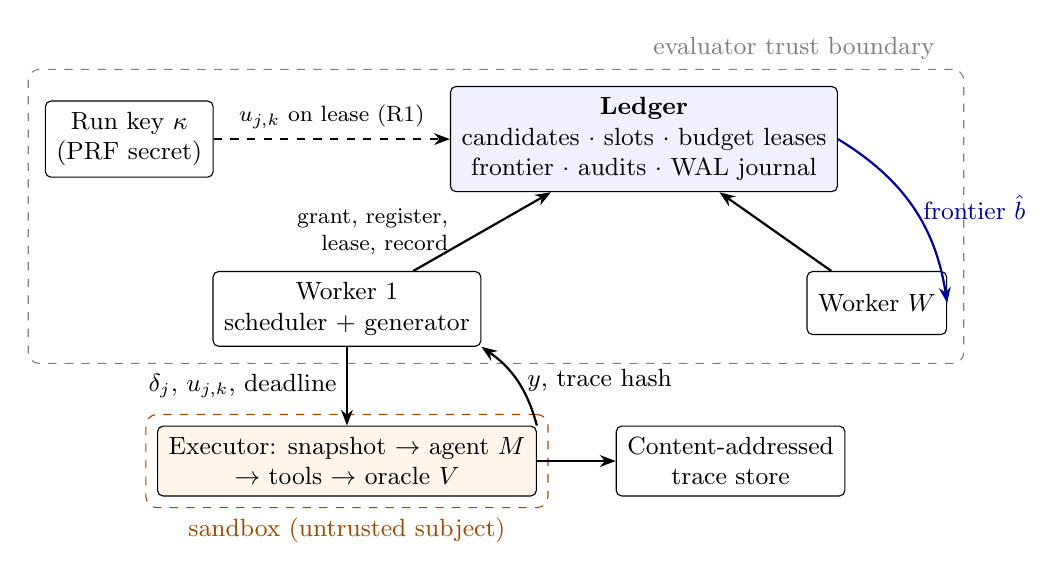
\begin{tikzpicture}[node distance=6mm and 10mm, every node/.style={font=\small},
  box/.style={draw, rounded corners=2pt, align=center, minimum height=8mm, inner sep=4pt},
  arr/.style={-{Stealth[length=2mm]}, thick}]
\node[box, fill=blue!6] (L) {\textbf{Ledger}\\ candidates $\cdot$ slots $\cdot$ budget leases\\ frontier $\cdot$ audits $\cdot$ WAL journal};
\node[box, left=30mm of L] (K) {Run key $\kappa$\\ (PRF secret)};
\node[box, below left=10mm and -4mm of L] (W1) {Worker 1\\ scheduler + generator};
\node[box, below right=10mm and -4mm of L] (W2) {Worker $W$};
\node[box, below=10mm of W1, fill=orange!8] (X) {Executor: snapshot $\to$ agent $M$\\ $\to$ tools $\to$ oracle $V$};
\node[box, right=10mm of X] (T) {Content-addressed\\ trace store};
\draw[arr, dashed] (K) -- node[above, font=\footnotesize]{$u_{j,k}$ on lease (R1)} (L);
\draw[arr] (W1) -- node[left=3mm, align=right, font=\footnotesize]{grant, register,\\ lease, record} (L);
\draw[arr] (W2) -- (L);
\draw[arr, blue!60!black] (L.east) to[bend left=25] node[right]{frontier $\bhat$} (W2.east);
\draw[arr] (W1) -- node[left]{$\delta_j$, $u_{j,k}$, deadline} (X);
\draw[arr] (X.north east) to[bend right=20] node[right]{$y$, trace hash} (W1.south east);
\draw[arr] (X) -- (T);
\begin{scope}[on background layer]
\node[draw=gray, dashed, rounded corners, fit=(L)(K)(W1)(W2), inner sep=6pt, label={[gray]above right:evaluator trust boundary}] {};
\node[draw=orange!60!black, dashed, rounded corners, fit=(X), inner sep=4pt, label={[orange!60!black]below:sandbox (untrusted subject)}] {};
\end{scope}
\end{tikzpicture}
\caption{Reference implementation. A single logical ledger enforces R1, R3, R5 and R6; workers and the frontier broadcast are soft state that affects only efficiency.}\label{fig:arch}
\end{figure}

The rules can be met in several ways; any harness that satisfies Table~\ref{tab:rules} inherits the guarantees. Our reference implementation (Fig.~\ref{fig:arch}) uses one logical ledger as the serialisation point. Its state (candidates, slots, budget leases, frontier, audits) changes only through journaled, atomic transitions---\textsc{Grant}, \textsc{Register}, \textsc{Lease}, \textsc{Record}, \textsc{Expire}, \textsc{Advance}, \textsc{Prune}, \textsc{Close}, \textsc{Audit}. Requests carry (sender, request id) with cached responses, so retransmissions are idempotent; slot results are fenced by lease tokens (R3); expired slots become non-violating records (R4) or, in replay mode, are re-leased with the same key; budget leases are bound to a worker incarnation and fenced on close (R5); and confirmation is recomputed from stored slots (R6). Invariants (budget conservation, write-once slots, monotone commit pointer and frontier, confirmation soundness) are checked after every transition in property-based tests, and journal replay reproduces the ledger state exactly after a coordinator crash.

\begin{algorithm}[!htbp]
\caption{Worker loop. Any scheduling policy is valid under Theorem~\ref{thm:seq}.}\label{alg:worker}
\begin{algorithmic}[1]
\Loop
\If{no open budget lease} \State request \textsc{Grant} \EndIf
\State $a\gets$ \Call{Schedule}{latest frontier, local state}
\If{$a=\textsc{New}(k)$} \State $\delta\gets G_k.\textsc{Propose}()$; \textsc{Register}(lease, $\delta$) \Comment{$a_j$ fixed here}
\ElsIf{$a=\textsc{Continue}(j,m)$}
  \For{each $(k,u,\text{tok})\in$ \textsc{Lease}$(j,m)$}
    \State $y\gets$ \textsc{Execute}$(\delta_j,u,\text{deadline})$; \textbf{if} no crash \textbf{then} \textsc{Record}$(j,k,y,\text{tok})$ \Comment{retried until acknowledged}
  \EndFor
\EndIf
\EndLoop
\end{algorithmic}
\end{algorithm}

A shared ledger is not the only way to satisfy R5: $W$ independent single-worker deployments with budget $\varepsilon/W$ each also comply. Section~\ref{sec:results} compares the two. Production deployments need no message broker, cache or custom consensus---a broker would add an at-least-once hop that must then be deduplicated---and task frameworks may place executors only with automatic retries disabled, since those retries implement the fresh-retry default.

% -----------------------------------------------------------------------------
\section{Evaluation methodology}\label{sec:method}

\paragraph{Why synthetic.} Validity claims need ground truth---which candidates are null and the true margin $k^*$---which real agents never provide. We use (a) a deterministic discrete-event simulator that runs the implemented ledger, message layer and workers with injected faults (loss, duplication, reordering, partitions, worker and executor crashes, ledger crash and journal recovery, outcome-correlated lognormal latency with means 20\,s benign and 30\,s violating) and Bernoulli oracles of known $p$; and (b) slot-level Monte Carlo of the confirmation procedures.

\paragraph{Instances.} Four cost levels; S1-moderate has violating fractions $(0,0,0.05,0.10)$ with $p=0.6$, S2-sparse $(0,0,0.01,0.05)$, and nulls with $p\sim U(0,0.2)$; the boundary null sets every candidate to $p=\alpha=0.2$, so every confirmation is false. $\alpha=0.2$, $\varepsilon=0.05$, four executors per worker.

\paragraph{Statistics.} Seeds are the unit of analysis. Validity is judged by Wilson intervals against $\varepsilon$; time-to-margin is censored at a common horizon and compared by restricted mean survival time with bootstrap intervals and Holm-corrected Mann--Whitney tests~\cite{kaplan1958}; non-inferiority uses Newcombe intervals for differences of proportions. Hypotheses and decision criteria were committed before the full runs (Table~\ref{tab:verdicts}); the fixed-sample rule study (Table~\ref{tab:fixed}) was added during this reframing and is not preregistered.

% -----------------------------------------------------------------------------
\section{Results}\label{sec:results}
All results are synthetic.

\subsection{The rules matter for both test families}
Through the full system (400 seeds per cell, boundary null, sequential confirmation), removing deduplication raised the false-confirmation probability to 0.133 [0.103, 0.169], allowing fresh-key retry to 0.102 [0.076, 0.136], and consuming results in arrival order to 0.083 [0.059, 0.114]; with all rules it stayed between 0.003 and 0.018 in every fault configuration, including all faults combined (0.003 [0.000, 0.014]). A worker-local budget at $W=8$ gave 0.065 [0.045, 0.094], an inflation not established at this configuration. For fixed-sample confirmation (Table~\ref{tab:fixed}) the defaults were at least as harmful: using the first $n$ results to arrive broke validity almost surely (0.999), fresh retry gave 0.189, duplicates 0.111, and a worker-local budget at $W=8$ 0.266; with the rules the rate stayed at or below 0.035.

\begin{table}[!htbp]\centering\small
\caption{Fixed-sample (exact Clopper--Pearson) confirmation of a 12-test family at the boundary null, $n=30$, level $\varepsilon/12$ per test (50,000 runs; 95\% Wilson intervals). Not preregistered.}\label{tab:fixed}
\begin{tabular}{lc}
\toprule
Configuration & $\Pr$(false confirmation) \\\midrule
Rules applied, no faults & 0.035 [0.034, 0.037] \\
Rules applied, crashes 0.3 / 0.1 imputed as non-violating & 0.014 [0.013, 0.015] \\
Rules applied, $W=8$ with one global budget & 0.019 [0.016, 0.023] \\\midrule
Default: duplicates counted (rate 0.3) & 0.111 [0.108, 0.114] \\
Default: crash $\to$ fresh-key retry & 0.189 [0.186, 0.193] \\
Default: first $n$ of $2n$ arrivals, violations faster & \textbf{0.999} [0.998, 0.999] \\
Default: worker-local budget, $W=8$ & 0.266 [0.255, 0.277] \\
\bottomrule\end{tabular}
\end{table}

\begin{figure}[!htbp]\centering
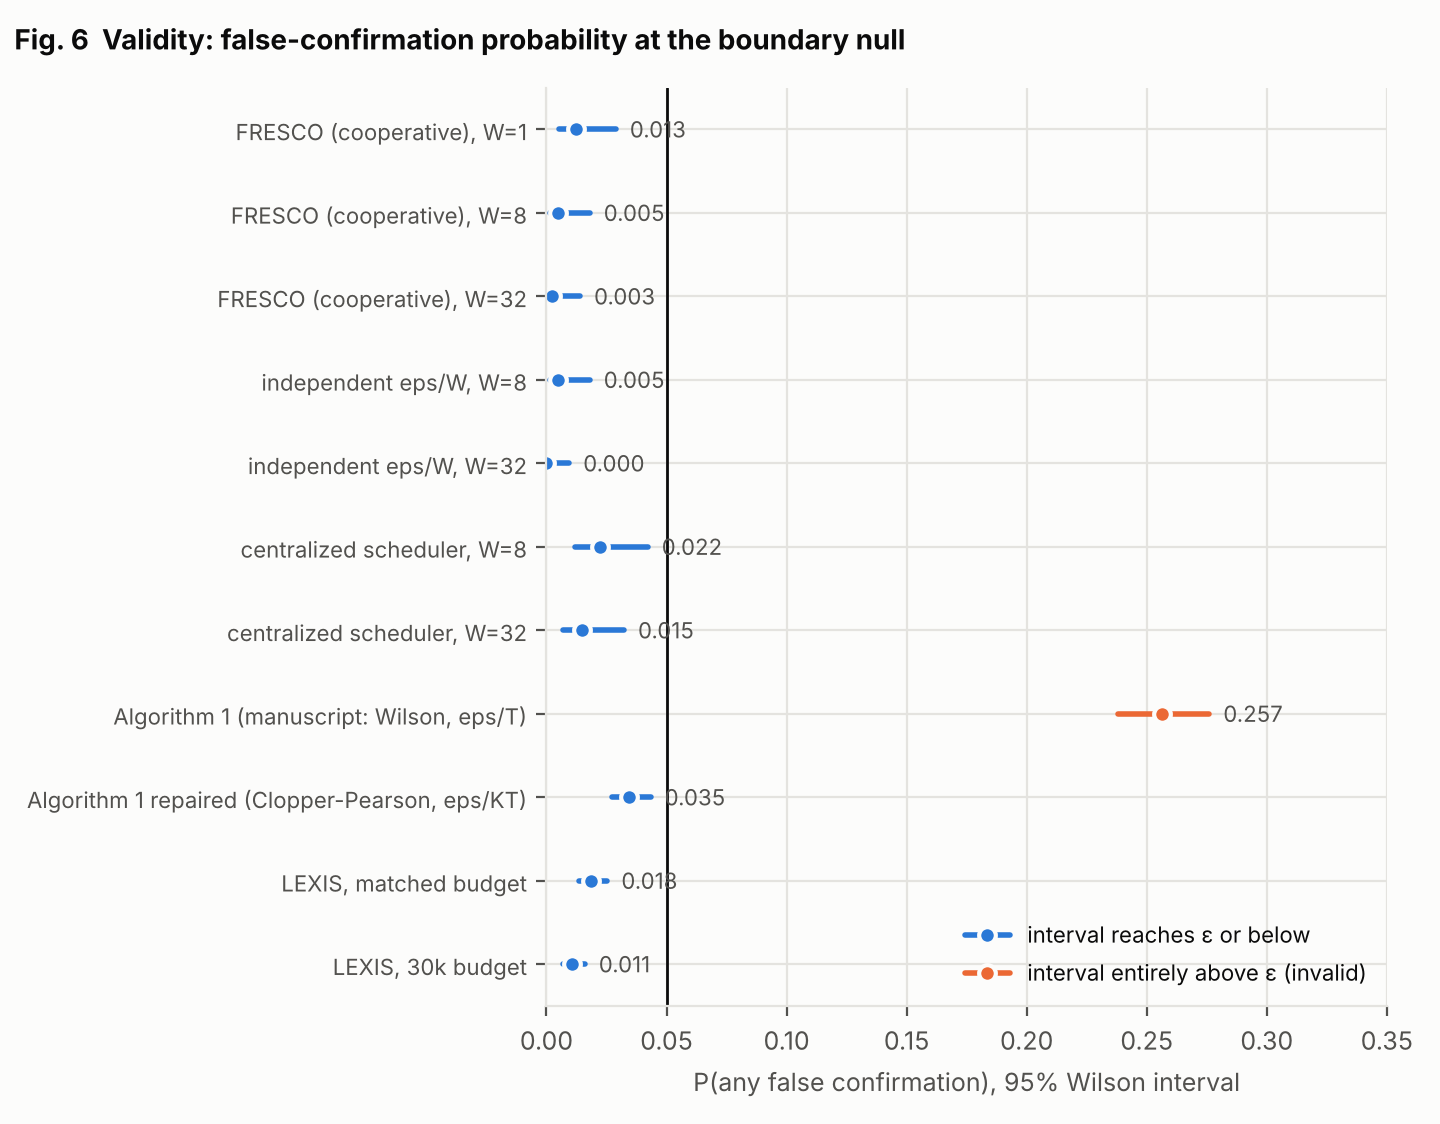
\includegraphics[width=0.82\linewidth]{fig6_validity.png}
\caption{False-confirmation probability at the boundary null for all procedures and deployments. Only Algorithm~1 as specified is invalid.}\label{fig:validity}
\end{figure}

\subsection{Audit of the MARGIN-Bench estimator}
As specified, Algorithm~1 confirmed a boundary-null candidate in 0.257 [0.238, 0.276] of 2,000 runs, five times its nominal level (Fig.~\ref{fig:validity}); the exact repair gave 0.035 [0.027, 0.043] with indistinguishable power (P(reach $k^*$) 0.800 versus 0.803 on S1).

\subsection{What the rules cost}
The reference implementation reached the true margin 25.4$\times$ faster with 32 workers than with one on S1 (parallel efficiency 0.79; at least 21.4$\times$ on S2, where single-worker runs were often censored) while the number of episodes needed stayed nearly flat (5.2k to 6.6k, overlapping intervals; Fig.~\ref{fig:scaling}). Coordination cost about 3.3--3.7 messages per episode and roughly 10 ledger operations per second at $W=32$ in virtual time. After a 60\,s ledger crash, a crash of half the workers or a 300\,s partition, throughput recovered within one 20\,s measurement bucket, and lost work matched the arithmetic loss. The main efficiency cost of the rules is conservative crash imputation: under 20\% crashes, time to the margin rose 1.7$\times$, mostly recovered by same-key replay.

\begin{figure}[!htbp]\centering
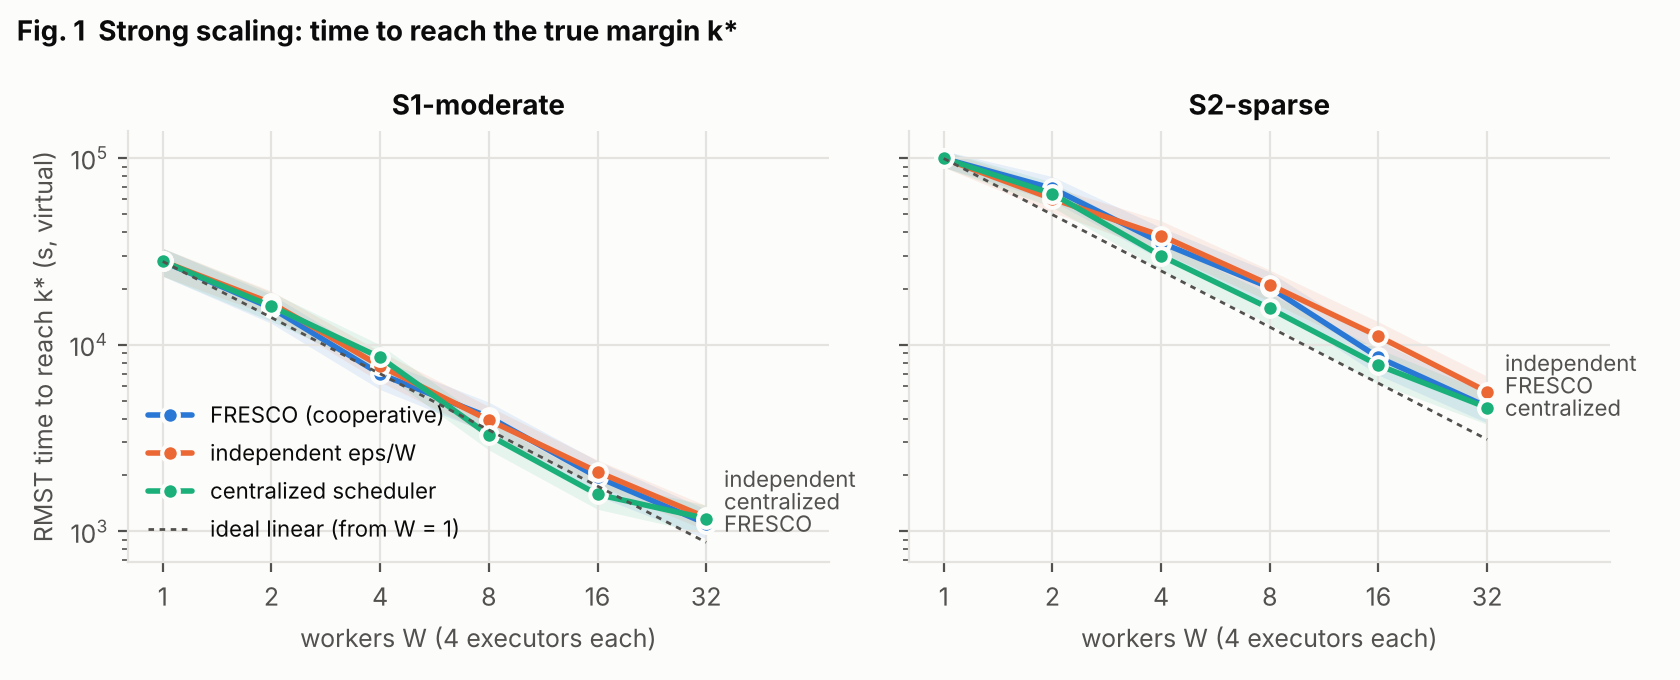
\includegraphics[width=\linewidth]{fig1_strong_scaling.png}
\caption{Time to reach the true margin versus workers for the shared-ledger deployment, $W$ independent deployments with budget $\varepsilon/W$, and one centralized scheduler (shaded: 95\% bootstrap CI). All three comply with the rules.}\label{fig:scaling}
\end{figure}

\subsection{Choosing a confirmation procedure}
At a matched budget of 1,160 episodes (Table~\ref{tab:eff}), repaired Algorithm~1 reached $k^*$ in 0.808 of S1 runs; LEXIS without screening reached it in only 0.246, because it runs every opened null candidate to its cap. Adding screening (LEXIS-S) lifted this to 0.756 (S1) and 0.251 (S2, versus 0.269), but the preregistered non-inferiority margin of 0.05 was met in only 2 of 6 parameter settings, total episodes were unchanged (screening dominates cost), and scouting-weighted spending gave no detectable benefit. LEXIS-S was markedly more conservative (0.004 false confirmations versus 0.034): an anytime-valid test capped at a fixed sample uses less of its error budget, and that unused budget is the power it gives up. With 5,000 episodes and repeated passes both procedures reached $k^*$ almost always on S1 (0.998, 1.000) and in 0.733 versus 0.765 of S2 runs.

\begin{table}[!htbp]\centering\small
\caption{Probability of reaching the true margin $k^*=3$ at a matched single-pass budget and with repeated passes (2,000 runs per cell; slot level). Rows 1 and 3 come from the first comparison (E4), the others from the preregistered hybrid study (E8); repaired Algorithm~1 was measured in both (S1: 0.800 and 0.808).}\label{tab:eff}
\begin{tabular}{lccc}
\toprule
Procedure & S1 & S2 & $\Pr$(false), boundary null \\\midrule
Algorithm 1 as specified (invalid) & 0.803 & 0.280 & 0.257 \\
Algorithm 1 repaired & \textbf{0.808} & \textbf{0.269} & 0.034 \\
LEXIS (no screening) & 0.246 & 0.043 & 0.018 \\
LEXIS-S (screening + e-process) & 0.756 & 0.251 & 0.004 \\\midrule
Algorithm 1 repaired, multi-pass (5,000) & 1.000 & 0.765 & 0.015 \\
LEXIS-S, multi-pass (5,000) & 0.998 & 0.733 & 0.014 \\
\bottomrule\end{tabular}
\end{table}

\subsection{Is a shared coordinator worth it?}
No measurable speed-up. In all 20 Holm-corrected comparisons (two instances, $W\in\{2,\dots,32\}$) the shared-ledger deployment was indistinguishable from $W$ independent $\varepsilon/W$ deployments and from one centralized scheduler: restricted-mean-time ratios 0.77--1.30, every 95\% CI containing 1, every adjusted $p\ge0.94$. With 100 seeds per cell, effects smaller than a ratio of about 0.65 could not be detected. Sharing one budget spreads it over more registrations, roughly cancelling the union-bound saving, while frontier pruning saves only work above the current margin.

\subsection{Certificates}
Per-level certificates covered the true violating mass in every run (coverage 1.000 [0.981, 1.000]) but were loose: median bounds of 0.39--0.75 against true masses of 0--0.01 after 100--280 audits per level. They are valid statements about the generator, not evidence of robustness.

\begin{table}[!htbp]\centering\small
\caption{Preregistered hypotheses and verdicts (synthetic evidence).}\label{tab:verdicts}
\begin{tabularx}{\linewidth}{lX>{\raggedright\arraybackslash}p{4.0cm}}
\toprule
Hypothesis & Criterion & Verdict \\\midrule
H-valid & Wilson lower bound $\le\varepsilon$ in all rule-compliant configurations & supported \\
H-rules & removing a rule gives lower bound $>\varepsilon$ (sequential, system level) & supported for 3 of 4 \\
H-alg1 & Algorithm 1 as specified exceeds $\varepsilon$; repair does not & supported \\
H-speed & speedup lower bound $\ge16$ at $W=32$ & supported (25.4$\times$) \\
H-overhead & $\le10$ messages per episode, $\le100$ ledger ops/s & supported \\
H-recover & 90\% throughput within $2\times$ outage & supported \\
H-coop & shared ledger faster than independent or centralized & \textbf{not supported} \\
H-vs-Alg1 & LEXIS reaches $k^*$ as often as repaired Algorithm 1 & \textbf{refuted} \\
H6-noninf & LEXIS-S within 0.05 of repaired Algorithm 1 & \textbf{not supported} (2/6 settings) \\
H6-cheaper & LEXIS-S uses fewer episodes & \textbf{refuted} (ratio $\approx1.00$) \\
H-cert & certificate coverage $\ge0.95$ & supported; bounds loose \\
H-valid-real & measured fault profiles imply inflation & \todo{TO RUN} \\
\bottomrule\end{tabularx}
\end{table}

\subsection{Real-agent experiments}\label{sec:real}
Not yet run. The protocol: (1) profile 2,000 episodes per open-weight model to estimate timeout and crash rates separately for violating and benign trajectories, and measure redelivery rates of common queue configurations; (2) re-run the fault-injection studies of Tables~\ref{tab:fixed} and the sequential ablations with the measured rates; (3) replay 200 completed slots to verify seeded determinism; (4) compare procedures on 20 MARGIN-Bench scenario families with cluster bootstrap over families; (5) report authorized-task completion on paired counterparts. Table~\ref{tab:real} lists the required evidence.

\begin{table}[!htbp]\centering\small
\caption{Real-agent result shells. No value may be filled except from executed runs.}\label{tab:real}
\begin{tabular}{lll}
\toprule
Quantity & Model A & Model B \\\midrule
Timeout/crash rate by outcome $(c_0,c_1)$ & \todo{TO RUN} & \todo{TO RUN} \\
Redelivery rate of the naive queue & \todo{TO RUN} & \todo{TO RUN} \\
Implied false-confirmation inflation per default & \todo{TO RUN} & \todo{TO RUN} \\
Replay determinism (\% trace-hash match) & \todo{TO RUN} & \todo{TO RUN} \\
Episodes to $\bhat$: repaired Algorithm 1 / LEXIS-S & \todo{TO RUN} & \todo{TO RUN} \\
Authorized-task completion & \todo{TO RUN} & \todo{TO RUN} \\
\bottomrule\end{tabular}
\end{table}

% -----------------------------------------------------------------------------
\section{Practitioner checklist}\label{sec:checklist}
\begin{enumerate}
\item Derive each episode's randomness from (run key, candidate, slot index); reveal it only when the slot is dispatched; publish a hash of the run key before the run.
\item Store results write-once per (candidate, slot) and ignore duplicates; never count a redelivered result.
\item Decide which slots form the evidence \emph{before} running them: the in-order prefix for sequential tests, a fixed index set for fixed-sample tests. Never use ``the first $n$ results to arrive''.
\item Record a crashed or timed-out episode as non-violating when confirming (violating when certifying absence); never silently re-run it with new randomness. Replay with the same key only after auditing determinism; disable automatic retries in task frameworks.
\item Spend one error budget across all workers, all budget levels and all passes; correct across levels.
\item Recompute every confirmation from stored records.
\item Reset all agent state (memory, tool state) between episodes, and audit the oracle for false positives.
\item Preregister deadlines, thresholds and test parameters, and report imputation rates per arm.
\end{enumerate}

% -----------------------------------------------------------------------------
\section{Discussion and failure analysis}\label{sec:discussion}

\paragraph{What the evidence supports.} Ordinary execution semantics can multiply the error of agent security evaluations, sometimes to certainty, and six cheap rules prevent it for both common families of confirmation tests. The rules cost one write per episode, scale near-linearly, and recover quickly from faults. The audit shows the issue is not hypothetical bookkeeping: a concrete, carefully specified benchmark estimator was invalid for the related reason of uncorrected multiplicity.

\paragraph{What it does not support.} A shared coordinator is not needed for speed: independent deployments with a split budget are as fast and equally valid, provided each follows the rules. Anytime-valid confirmation is not more sample-efficient: at a fixed budget the repaired fixed design is slightly more powerful, and early stopping saves little when screening dominates cost. Sequential confirmation remains the right choice when runs must be extended or stopped unpredictably.

\paragraph{When the guarantees fail.} Shared hidden state between episodes (e.g.\ agent memory not reset) violates Assumption~\ref{as:a1} and can inflate error under any execution; oracle false positives shift the guarantee to the observed rate; leaked keys enable selection on seeds. If violating episodes time out more often than benign ones, conservative imputation hides them: validity holds but power collapses, so deadlines are statistical parameters to be preregistered.

% -----------------------------------------------------------------------------
\section{Threats to validity}\label{sec:threats}
\textit{Construct:} the fault rates are chosen triggers, not measurements; real harnesses may show smaller (or larger) effects. \textit{Internal:} procedure parameters were not tuned beyond a small preregistered sweep; one LEXIS variant is labelled exploratory; the fixed-sample rule study was added during reframing. \textit{Statistical:} 400 runs per system-level cell limit detection of modest inflation, which is why the global-budget result remains open at $W=8$; seeds share random streams across methods. \textit{External:} simulated generators are non-adaptive and instances small. \textit{Implementation:} the database-backed ledger is specified but not executed; coordination cost is measured in virtual time.

\section{Limitations and negative results}\label{sec:limits}
(i) No real-agent results. (ii) No speed-up from a shared coordinator. (iii) Sequential confirmation, with or without screening, is somewhat less powerful than a repaired fixed design at a fixed budget. (iv) Certificates are loose at realistic audit budgets. (v) The necessity of the global budget was not established at $W=8$ at system level for sequential tests (it was for fixed-sample tests). (vi) Byzantine executors are not covered. (vii) Bit-reproducible epoch mode and a database adapter are not implemented.

\section{Reproducibility and data availability}\label{sec:repro}
Code, configurations, raw results (JSON lines with configuration hashes and code revisions), analysis scripts and figures are in the project repository \todo{INSERT PERMANENT ARCHIVE DOI}. One script regenerates every result in about two hours on four cores; 46 unit, property-based and integration tests cover the ledger, protocol, procedures and simulator; the simulator is deterministic given configuration and seed.

\section{Future work}\label{sec:future}
Execute the real-agent protocol; measure the rules' effect in widely used open-source evaluation harnesses; extend the rules to estimators with adaptive allocation of confirmation trials and to Byzantine executors with attestation; and narrow the power gap of anytime-valid confirmation at fixed budgets.

\section{Conclusion}\label{sec:conclusion}
The error level of an agent security evaluation is a property of the whole experiment, including how its harness delivers, retries, orders and budgets episodes. We gave six rules that make sequential and fixed-sample confirmation valid under the faults of real infrastructure, showed that each common default can break validity, repaired an estimator that was invalid as specified, and found that the rules are cheap while a shared coordinator and anytime-valid confirmation buy flexibility rather than speed or power. Real-agent measurements remain to be done.

% -----------------------------------------------------------------------------
\section*{Declarations}
\noindent\textbf{Funding.} \todo{INSERT TRUE FUNDING INFORMATION OR ``No funding was received''.}\\
\textbf{Competing interests.} \todo{AUTHORS TO DISCLOSE.}\\
\textbf{Ethics approval.} Not applicable to the simulation study; the real-agent protocol uses sandboxed mock tools and no human participants \todo{CONFIRM BEFORE REAL-AGENT RUNS}.\\
\textbf{Data availability.} Synthetic results are released with the code \todo{ARCHIVE DOI}. No real-agent data exist yet.\\
\textbf{Code availability.} \todo{REPOSITORY URL AND ARCHIVE DOI}.\\
\textbf{Author contributions.} \todo{CRediT STATEMENT}.\\
\textbf{Use of generative AI.} \todo{AUTHORS MUST DISCLOSE: substantial parts of the design, code, analysis and text of this working manuscript were drafted with an AI assistant and must be verified and declared according to the journal's policy.}

\bibliographystyle{unsrtnat}
\bibliography{references}
\end{document}
